\documentclass[12pt,a4paper,oneside]{report}
\usepackage{examgrid}
\setdoc{Mini Project Report}{CS3603-1}
\newcommand{\src}{../../src/main/java/com/examgrid}

\titleformat{\chapter}[display]{\normalfont\bfseries\color{egnavy}}{\large CHAPTER \thechapter}{4pt}{\LARGE}
\titlespacing*{\chapter}{0pt}{-10pt}{18pt}

\begin{document}
\nmamitcover{Mini Project Report}{Submitted in partial fulfilment of the requirements of\\Java and Spring Framework Laboratory (CS3603-1)\\Bachelor of Technology in Computer Science and Engineering}{\small Under the guidance of\\[2pt]\textbf{\rule{6cm}{0.4pt}}\\Department of Computer Science and Engineering\\[6pt]November 2026}

\pagenumbering{roman}
\thispagestyle{plain}
\begin{center}
{\large\bfseries NMAM INSTITUTE OF TECHNOLOGY, NITTE}\\[2pt]
Department of Computer Science and Engineering\\[1.2cm]
{\Large\bfseries\color{egnavy} CERTIFICATE}
\end{center}
\vspace{0.6cm}
\noindent Certified that the mini project work entitled \textbf{``ExamGrid: An Automated Exam Seating and Invigilation Allocation System using Spring Boot''} is a bona fide work carried out by
\begin{center}
\begin{tabular}{l l}
Prajwal Jogi & NNM25CS522\\
Prajwal Acharya & NNM25CS521\\
Sathwik P Shetty & NNM24CS224\\
Satvik Hegde & NNM24CS225\\
\end{tabular}
\end{center}
\noindent in partial fulfilment of the requirements of the Java and Spring Framework Laboratory (CS3603-1) of the V semester B.Tech in Computer Science and Engineering during the academic year 2026--27. The mini project report has been approved as it satisfies the academic requirements in respect of the laboratory work prescribed for the said course.
\vspace{2.5cm}

\noindent\begin{tabular}{@{}p{7cm}p{7cm}@{}}
\rule{5cm}{0.4pt} & \rule{5cm}{0.4pt}\\
Signature of the Course Instructor & Signature of the HOD\\
\end{tabular}
\vspace{2cm}

\noindent\begin{tabular}{@{}p{7cm}p{7cm}@{}}
Name of the Examiners & Signature with Date\\[0.8cm]
1. \rule{5cm}{0.4pt} & \rule{5cm}{0.4pt}\\[0.8cm]
2. \rule{5cm}{0.4pt} & \rule{5cm}{0.4pt}\\
\end{tabular}
\newpage

\thispagestyle{plain}
\begin{center}{\Large\bfseries\color{egnavy} DECLARATION}\end{center}
\vspace{0.5cm}
We hereby declare that the mini project entitled \textbf{``ExamGrid: An Automated Exam Seating and Invigilation Allocation System using Spring Boot''} submitted to the Department of Computer Science and Engineering, NMAM Institute of Technology, Nitte, is a record of the work carried out by us during the V semester of the academic year 2026--27 as part of the course CS3603-1. The work has not been submitted elsewhere for the award of any degree or credit.
\vspace{2cm}

\noindent\begin{tabular}{@{}p{5.5cm}p{3.5cm}p{4cm}@{}}
Prajwal Jogi & NNM25CS522 & \rule{3.5cm}{0.4pt}\\[0.7cm]
Prajwal Acharya & NNM25CS521 & \rule{3.5cm}{0.4pt}\\[0.7cm]
Sathwik P Shetty & NNM24CS224 & \rule{3.5cm}{0.4pt}\\[0.7cm]
Satvik Hegde & NNM24CS225 & \rule{3.5cm}{0.4pt}\\
\end{tabular}

\vspace{1cm}\noindent Place: Nitte\\Date: \rule{3cm}{0.4pt}
\newpage

\thispagestyle{plain}
\begin{center}{\Large\bfseries\color{egnavy} ACKNOWLEDGEMENT}\end{center}
\vspace{0.5cm}
We express our sincere gratitude to our course instructor for the Java and Spring Framework Laboratory for the guidance, encouragement and valuable feedback given throughout this mini project.

We thank the Head of the Department of Computer Science and Engineering for providing the laboratory facilities and an environment that encouraged us to complete this work.

We are grateful to the Principal, NMAM Institute of Technology, Nitte, for the support extended to the students.

We also thank the staff of the examination cell for explaining the present seating and invigilation process, which helped us understand the real requirements of the system.

Finally, we thank our parents and friends for their constant support.
\vspace{1cm}

\hfill Prajwal Jogi\\
\hspace*{\fill} Prajwal Acharya\\
\hspace*{\fill} Sathwik P Shetty\\
\hspace*{\fill} Satvik Hegde
\newpage

\thispagestyle{plain}
\begin{center}{\Large\bfseries\color{egnavy} ABSTRACT}\end{center}
\vspace{0.3cm}
Allocating examination halls, seats and invigilators is still done manually in many institutions, usually on spreadsheets. The process takes hours and is error-prone: students of the same subject end up sitting side by side, halls get over-filled, and faculty receive overlapping duties or an uneven workload. ExamGrid is a Spring Boot web application that automates this entire workflow. The exam cell registers exams, halls (with their row-column layout), students and faculty. A rule-based allocation engine then generates a conflict-free seating plan that spreads students of the same subject and branch across benches and respects hall capacity. It also assigns invigilators with balanced workload and no time clashes. Students can look up their hall and seat number using their USN, faculty can view their duty roster, and the exam cell can export printable seating charts and duty lists.

The system follows a layered MVC architecture. It uses Spring MVC with Thymeleaf for the user interface and Spring Data JPA with Hibernate for persistence in MySQL. RESTful APIs, tested with Postman and curl, serve seat lookup and roster data. It also includes role-based login with session management, server-side validation, and centralized exception handling for cases such as record not found or insufficient hall capacity. On the sample data of 148 students, four halls and ten faculty, the engine seats every student with zero same-subject neighbours and assigns fourteen invigilation duties with no clashes and a workload difference of at most one duty, replacing hours of manual planning with an operation that completes in well under a second.

\vspace{0.3cm}\noindent\textbf{Keywords:} Spring Boot, Spring MVC, Thymeleaf, Spring Data JPA, Hibernate, MySQL, REST API, exam seating allocation, invigilation scheduling.
\newpage

\tableofcontents
\listoffigures
\listoftables
\newpage
\pagenumbering{arabic}

\chapter{Introduction}
\section{Overview}
Examinations are conducted several times every semester -- two internal assessments and the semester-end examination -- and for each examination session the examination cell must decide where every student sits and which faculty member supervises each hall. In most colleges this planning is done in spreadsheets by copying student lists into hall layouts. ExamGrid replaces this manual work with a web application built on the Spring Framework.

\section{Problem Statement}
Design and implement a web application that automatically generates a conflict-free examination seating plan and a balanced, clash-free invigilation duty roster from the exam timetable, hall layouts, student list and faculty list, and that lets students and faculty look up their allocations online.

\section{Objectives}
\begin{enumerate}
  \item Maintain students, faculty, halls and exams through a secure web interface.
  \item Generate seating that respects hall capacity and keeps students of the same subject apart.
  \item Assign invigilators without time clashes and with balanced workload.
  \item Provide seat lookup by USN and duty rosters through REST APIs and the Fetch API.
  \item Produce printable PDF seating charts and duty rosters.
  \item Apply Spring Boot, Spring MVC, Thymeleaf, Spring Data JPA, Spring Security, Bean Validation and \texttt{@ControllerAdvice} in one complete project.
\end{enumerate}

\section{Scope}
The project covers master data management, seating and invigilation allocation, PDF export, online lookup, a REST API and role-based security. Question papers, results and notifications are outside the scope.

\section{Organization of the Report}
Chapter 2 reviews the existing system. Chapter 3 lists the requirements. Chapter 4 explains the design and database. Chapter 5 describes the allocation algorithms. Chapter 6 covers the implementation, Chapter 7 the REST API and testing, and Chapter 8 the results with screenshots. Chapter 9 concludes the report and lists future enhancements.

\chapter{Literature Survey and Existing System}
\section{Existing Manual System}
\begin{itemize}
  \item Student lists are exported from the university portal and pasted into spreadsheet templates of each hall.
  \item Mixing of subjects is done by hand, for example by alternating two branches column by column.
  \item Invigilation duties are assigned from a faculty list, often in the order of the list, and clashes are checked by eye.
  \item Seat charts are printed and pasted outside halls; students crowd around notice boards before the exam.
\end{itemize}
\section{Drawbacks}
\begin{itemize}
  \item Time consuming: several hours per exam day, repeated for every timetable change.
  \item Error prone: over-filled halls, students of the same subject side by side, duplicate seats.
  \item Unfair workload: some faculty receive many more duties than others; overlapping duties are discovered late.
  \item No self-service: students and faculty depend on notice boards and circulars.
\end{itemize}
\section{Related Work}
Exam seating and invigilator assignment are studied in operations research as variants of the \emph{graph colouring} and \emph{assignment} problems. Exact formulations using integer linear programming or constraint programming give optimal answers but need specialised solvers and long running times for large inputs. Many practical systems use \emph{greedy heuristics} -- such as placing the largest remaining group first and checking only already-placed neighbours -- because they are fast, simple and produce conflict-free plans in typical college settings. Commercial examination management modules in ERP products include seating features but are expensive and not adaptable to a department's own rules. ExamGrid follows the greedy approach and implements it transparently in two small Java service classes.
\section{Proposed System}
ExamGrid automates the complete workflow: the exam cell enters master data once, generates the seating and invigilation plan per slot with a click, and publishes it instantly. Students and faculty see their allocation online, and printable PDFs are produced from the same data, so all copies are always consistent.

\chapter{Requirement Specification}
\section{Functional Requirements}
\begin{tabularx}{\linewidth}{|l|X|}
\hline\headrow\thead{Module} & \thead{Requirements}\\\hline
Authentication & Login for ADMIN, FACULTY and STUDENT; BCrypt passwords; role-based pages; one session per user.\\\hline
Master data & CRUD of students, faculty, halls and exams with validation; unique USN, faculty code and hall name; exam timing checks.\\\hline
Seating & Generate per slot; every student exactly once; within capacity; no same-subject neighbours when space allows; prefer different branches; report unavoidable clashes.\\\hline
Invigilation & After seating; $\lceil s/30\rceil$ per hall; no time clash; respect maximum duties; least-loaded first; all-or-nothing.\\\hline
Lookup and reports & Public seat lookup by USN; own seats for students; own duties for faculty; PDF seating chart and duty roster.\\\hline
REST API & JSON endpoints for all operations with uniform error responses.\\\hline
\end{tabularx}
\section{Non-Functional Requirements}
Performance (allocation of 1000 students in under 3 s), security (authentication, CSRF, session fixation protection), reliability (transactional allocation), usability (responsive pages), maintainability (layered code), testability (automated tests). The complete numbered list with 46 functional and 10 non-functional requirements is given in Document 01 (SRS).
\section{Hardware and Software Requirements}
\begin{tabularx}{\linewidth}{|l|X|}
\hline\headrow\thead{Item} & \thead{Requirement}\\\hline
Processor / RAM & Any dual-core processor, 4 GB RAM (2 GB free for the application)\\\hline
Operating system & Windows 10/11, Ubuntu 20.04+ or macOS\\\hline
Java & JDK 17 or newer\\\hline
Build tool & Apache Maven 3.9\\\hline
Database & MySQL Server 8.0\\\hline
IDE & IntelliJ IDEA / Eclipse / VS Code with Spring Boot extensions\\\hline
Browser & Chrome, Edge or Firefox (latest)\\\hline
Testing & Postman, curl, JUnit 5\\\hline
\end{tabularx}
\section{Use Cases}
\begin{figure}[H]\centering
\resizebox{0.92\linewidth}{!}{\begin{tikzpicture}[
  font=\footnotesize,
  uc/.style={ellipse,draw=egnavy,fill=eglight,minimum width=3.6cm,minimum height=0.75cm,align=center,inner sep=1pt},
  actor/.style={align=center,font=\footnotesize\bfseries},
  ln/.style={thick,eggrey}]
\newcommand{\stick}[2]{%
  \begin{scope}[shift={#1}]
  \draw[thick,egnavy] (0,0.55) circle (0.18);
  \draw[thick,egnavy] (0,0.37)--(0,-0.15) (-0.3,0.2)--(0.3,0.2) (0,-0.15)--(-0.22,-0.55) (0,-0.15)--(0.22,-0.55);
  \node[actor] at (0,-0.85) {#2};
  \end{scope}}
\draw[rounded corners=6pt,draw=egnavy,thick,fill=white] (-3.6,-7.4) rectangle (3.6,4.0);
\node[font=\bfseries,egnavy] at (0,3.65) {ExamGrid System};
\node[uc] (u1) at (0,3.0) {Login / Logout};
\node[uc] (u2) at (0,2.1) {Manage Students};
\node[uc] (u3) at (0,1.2) {Manage Faculty};
\node[uc] (u4) at (0,0.3) {Manage Halls};
\node[uc] (u5) at (0,-0.6) {Schedule Exams};
\node[uc] (u6) at (0,-1.5) {Generate Seating Plan};
\node[uc] (u7) at (0,-2.4) {Assign Invigilators};
\node[uc] (u8) at (0,-3.3) {Export PDF Charts};
\node[uc] (u9) at (0,-4.2) {View Duty Roster};
\node[uc] (u10) at (0,-5.1) {Look up Seat by USN};
\node[uc] (u11) at (0,-6.0) {View Own Seats};
\node[uc,fill=eggold!20,draw=eggold] (u12) at (0,-6.9) {Call REST API};
\stick{(-6,0.6)}{Exam Cell\\(ADMIN)}
\stick{(6,-3.6)}{Faculty}
\stick{(6,-0.6)}{Student}
\stick{(-6,-5.4)}{Guest /\\Postman}
\foreach \u in {u1,u2,u3,u4,u5,u6,u7,u8,u9,u12} \draw[ln] (-5.6,0.6)--(\u.west);
\foreach \u in {u1,u9} \draw[ln] (5.6,-3.6)--(\u.east);
\foreach \u in {u1,u10,u11} \draw[ln] (5.6,-0.6)--(\u.east);
\foreach \u in {u10,u12} \draw[ln] (-5.6,-5.4)--(\u.west);
\draw[-{Stealth},dashed,eggrey] (u7.east) to[out=0,in=0] node[right,font=\tiny]{$\langle\langle$requires$\rangle\rangle$} (u6.east);
\end{tikzpicture}
}
\caption{Use case diagram of ExamGrid}
\end{figure}

\chapter{System Design}
\section{Architecture}
ExamGrid follows the layered MVC architecture of Spring Boot (Figure~\ref{fig:arch5}). Requests pass through two Spring Security filter chains -- HTTP Basic for \texttt{/api/**} and form login with sessions for the web pages -- and reach either a \texttt{@Controller} that returns a Thymeleaf view or a \texttt{@RestController} that returns JSON. Controllers delegate to \texttt{@Service} classes, which hold all business rules and use Spring Data JPA repositories to access MySQL.
\begin{figure}[H]\centering
\resizebox{0.82\linewidth}{!}{\begin{tikzpicture}[
  font=\small,
  layer/.style={draw=egnavy,fill=eglight,rounded corners=3pt,minimum width=9.6cm,minimum height=1.05cm,align=center},
  comp/.style={draw=egnavy,fill=white,rounded corners=2pt,minimum height=0.7cm,align=center,font=\footnotesize},
  side/.style={draw=eggold,fill=eggold!15,rounded corners=3pt,minimum width=3.0cm,minimum height=1.05cm,align=center,font=\footnotesize},
  arr/.style={-{Stealth[length=2.5mm]},thick,egnavy}]

\node[layer,fill=white] (client) {\textbf{Client Tier} -- Web browser (Admin / Faculty / Student), Postman, curl};
\node[layer,below=0.55cm of client,fill=eggold!20,draw=eggold] (sec) {\textbf{Spring Security Filter Chains}\\[-1pt]\footnotesize API chain (/api/**, HTTP Basic) \quad Web chain (form login, session)};
\node[layer,below=0.55cm of sec,minimum height=1.6cm] (ctl) {};
\node[anchor=north] at (ctl.north) {\textbf{Controller Layer}};
\node[comp,anchor=south west] at ([xshift=0.25cm,yshift=0.15cm]ctl.south west) {Web Controllers\\(@Controller)};
\node[comp,anchor=south] at ([yshift=0.15cm]ctl.south) {REST Controllers\\(@RestController)};
\node[comp,anchor=south east] at ([xshift=-0.25cm,yshift=0.15cm]ctl.south east) {@ControllerAdvice\\handlers};
\node[layer,below=0.55cm of ctl,minimum height=1.6cm] (svc) {};
\node[anchor=north] at (svc.north) {\textbf{Service Layer} (@Service, @Transactional)};
\node[comp,anchor=south west] at ([xshift=0.2cm,yshift=0.15cm]svc.south west) {SeatingAllocation\\Service};
\node[comp,anchor=south] at ([xshift=-0.15cm,yshift=0.15cm]svc.south) {InvigilationAllocation\\Service};
\node[comp,anchor=south east] at ([xshift=-0.2cm,yshift=0.15cm]svc.south east) {CRUD + ReportPdf\\Services};
\node[layer,below=0.55cm of svc] (repo) {\textbf{Repository Layer} -- Spring Data JPA interfaces (JpaRepository)};
\node[layer,below=0.55cm of repo] (orm) {\textbf{Persistence} -- Hibernate ORM \,+\, JDBC (MySQL Connector/J)};
\node[layer,below=0.55cm of orm,fill=egnavy,text=white] (db) {\textbf{MySQL 8} -- examgrid\_db};

\node[side,right=0.6cm of ctl] (view) {\textbf{View}\\Thymeleaf templates\\Bootstrap 5, JS Fetch};
\node[side,right=0.6cm of svc] (pdf) {\textbf{OpenPDF}\\Seating charts\\Duty rosters};
\node[side,right=0.6cm of repo] (ent) {\textbf{Model}\\JPA Entities\\DTO records};

\draw[arr] (client) -- node[right,font=\scriptsize]{HTTP request} (sec);
\draw[arr] (sec) -- (ctl);
\draw[arr] (ctl) -- (svc);
\draw[arr] (svc) -- (repo);
\draw[arr] (repo) -- (orm);
\draw[arr] (orm) -- (db);
\draw[arr,dashed] (ctl) -- (view);
\draw[arr,dashed] (svc) -- (pdf);
\draw[arr,dashed] (repo) -- (ent);
\draw[arr,eggold] (view.north) |- node[pos=0.25,right,font=\scriptsize]{HTML / JSON} (client.east);
\end{tikzpicture}
}
\caption{Layered architecture}\label{fig:arch5}
\end{figure}

\section{Database Design}
The database \texttt{examgrid\_db} contains seven tables. \texttt{seat\_allocations} is an associative entity linking a student, an exam and a hall with the seat position; \texttt{invigilation\_duties} links a faculty member and a hall with a time window. Unique constraints prevent the same student being seated twice in an exam and the same physical seat being used twice in a slot.
\begin{figure}[H]\centering
\resizebox{\linewidth}{!}{\begin{tikzpicture}[
  font=\scriptsize,
  ent/.style={rectangle split,rectangle split parts=2,draw=egnavy,thick,rounded corners=2pt,
              rectangle split part fill={egnavy,white},text width=3.25cm,align=left,inner sep=3pt},
  rel/.style={diamond,draw=eggold,fill=eggold!20,thick,aspect=2.2,inner sep=1pt,font=\scriptsize\itshape},
  ln/.style={thick,egnavy!80}]

\node[ent] (student) at (0,0) {\textcolor{white}{\textbf{STUDENTS}}\nodepart{two}
  \underline{id} BIGINT PK\\ usn VARCHAR(15) UK\\ name VARCHAR(80)\\ branch VARCHAR(10)\\ semester INT\\ email VARCHAR(100)};
\node[ent] (exam) at (0,-6.2) {\textcolor{white}{\textbf{EXAMS}}\nodepart{two}
  \underline{id} BIGINT PK\\ subject\_code VARCHAR(15)\\ subject\_name VARCHAR(100)\\ branch VARCHAR(10)\\ semester INT\\ exam\_date DATE\\ start\_time TIME\\ end\_time TIME};
\node[ent] (seat) at (6,-3.1) {\textcolor{white}{\textbf{SEAT\_ALLOCATIONS}}\nodepart{two}
  \underline{id} BIGINT PK\\ exam\_id FK\\ student\_id FK\\ hall\_id FK\\ exam\_date DATE\\ start\_time TIME\\ seat\_row INT\\ seat\_column INT\\ seat\_number VARCHAR(20)};
\node[ent] (hall) at (12,-3.1) {\textcolor{white}{\textbf{HALLS}}\nodepart{two}
  \underline{id} BIGINT PK\\ hall\_name VARCHAR(30) UK\\ block VARCHAR(30)\\ total\_rows INT\\ total\_columns INT};
\node[ent] (duty) at (12,-8.4) {\textcolor{white}{\textbf{INVIGILATION\_DUTIES}}\nodepart{two}
  \underline{id} BIGINT PK\\ faculty\_id FK\\ hall\_id FK\\ exam\_date DATE\\ start\_time TIME\\ end\_time TIME};
\node[ent] (faculty) at (5.5,-9.6) {\textcolor{white}{\textbf{FACULTY}}\nodepart{two}
  \underline{id} BIGINT PK\\ faculty\_code VARCHAR(15) UK\\ name VARCHAR(80)\\ department VARCHAR(10)\\ email VARCHAR(100)\\ max\_duties INT};
\node[ent] (user) at (12,1.2) {\textcolor{white}{\textbf{APP\_USERS}}\nodepart{two}
  \underline{id} BIGINT PK\\ username VARCHAR(30) UK\\ password VARCHAR(255)\\ role ENUM\\ enabled BIT};

\node[rel] (r1) at (3.4,-0.6) {allotted};
\node[rel] (r2) at (3.4,-6.0) {seats};
\node[rel] (r3) at (9.2,-2.0) {in};
\node[rel] (r4) at (12,-5.9) {covers};
\node[rel] (r5) at (9.0,-9.3) {performs};

\draw[ln] (student.east) -- node[above,pos=0.2]{1} (r1) -- node[above,pos=0.8]{N} (seat.north west);
\draw[ln] (exam.east) -- node[above,pos=0.2]{1} (r2) -- node[above,pos=0.8]{N} (seat.south west);
\draw[ln] (hall.west) -- node[above,pos=0.2]{1} (r3) -- node[above,pos=0.8]{N} (seat.east);
\draw[ln] (hall.south) -- node[right,pos=0.2]{1} (r4) -- node[right,pos=0.8]{N} (duty.north);
\draw[ln] (faculty.east) -- node[above,pos=0.2]{1} (r5) -- node[above,pos=0.8]{N} (duty.west);
\draw[ln,dashed,eggrey] (user.west) -- node[above,font=\tiny,align=center]{username = usn}  (student.north east);
\node[font=\tiny,eggrey,align=center,below=1pt of user] {login account: username = USN (student)\\or faculty\_code (faculty) or ADMIN};
\end{tikzpicture}
}
\caption{Entity-relationship diagram}
\end{figure}

\begin{table}[H]\centering\small
\caption{Summary of tables}
\begin{tabularx}{\linewidth}{|l|X|}
\hline\headrow\thead{Table} & \thead{Main columns}\\\hline
students & id, usn (unique), name, branch, semester, email\\\hline
faculty & id, faculty\_code (unique), name, department, email, max\_duties\\\hline
halls & id, hall\_name (unique), block, total\_rows, total\_columns\\\hline
exams & id, subject\_code, subject\_name, branch, semester, exam\_date, start\_time, end\_time\\\hline
seat\_allocations & id, exam\_id, student\_id, hall\_id, exam\_date, start\_time, seat\_row, seat\_column, seat\_number\\\hline
invigilation\_duties & id, faculty\_id, hall\_id, exam\_date, start\_time, end\_time\\\hline
app\_users & id, username (unique), password (BCrypt), role, enabled\\\hline
\end{tabularx}
\end{table}
The schema is in third normal form; capacity is derived (rows $\times$ columns) rather than stored. The detailed data dictionary is in Document 02.

\section{Interaction Design}
\begin{figure}[H]\centering
\resizebox{\linewidth}{!}{\begin{tikzpicture}[font=\scriptsize,
  head/.style={draw=egnavy,fill=eglight,rounded corners=2pt,minimum width=2.1cm,minimum height=0.65cm,align=center,font=\scriptsize\bfseries},
  msg/.style={-{Stealth[length=2mm]},thick},
  ret/.style={-{Stealth[length=2mm]},dashed}]
\foreach \x/\n/\t in {0/b/Browser\\(seat-lookup.js),3.1/f/Security\\Filter,6.2/c/SeatLookup\\ApiController,9.3/s/SeatingAllocation\\Service,12.4/r/SeatAllocation\\Repository,15.2/d/MySQL}{
  \node[head] (\n) at (\x,0) {\t};
  \draw[eggrey,dashed] (\n.south) -- ++(0,-7.1);
}
\draw[msg] (0,-1.0) -- node[above]{GET /api/seats/NNM24CS224} (3.1,-1.0);
\draw[msg] (3.1,-1.5) -- node[above]{permitAll} (6.2,-1.5);
\draw[msg] (6.2,-2.0) -- node[above]{findSeatsByUsn(usn)} (9.3,-2.0);
\draw[msg] (9.3,-2.5) -- node[above]{existsByUsnIgnoreCase} (12.4,-2.5);
\draw[msg] (12.4,-2.9) -- node[above]{SELECT} (15.2,-2.9);
\draw[msg] (9.3,-3.5) -- node[above]{findByUsn (join fetch)} (12.4,-3.5);
\draw[msg] (12.4,-3.9) -- node[above]{SELECT ... JOIN} (15.2,-3.9);
\draw[ret] (15.2,-4.4) -- node[above]{rows} (12.4,-4.4);
\draw[ret] (12.4,-4.8) -- node[above]{List$<$SeatAllocation$>$} (9.3,-4.8);
\draw[ret] (9.3,-5.3) -- node[above]{List$<$SeatInfo$>$ (DTO)} (6.2,-5.3);
\draw[ret] (6.2,-5.8) -- node[above]{200 OK, JSON array} (0,-5.8);
\draw[msg] (0,-6.3) -- ++(0.6,0) -- ++(0,-0.35) node[right]{render seat cards (DOM)} -- ++(-0.6,0);
\node[draw=red!60!black,fill=red!6,font=\tiny,align=left,text width=3.1cm] at (8.0,-6.75) {alt: unknown USN $\rightarrow$ ResourceNotFound\-Exception $\rightarrow$ ApiExceptionHandler $\rightarrow$ 404 JSON};
\end{tikzpicture}
}
\caption{Sequence diagram of seat lookup}
\end{figure}

\chapter{Allocation Algorithms}
\section{Seating Allocation}
Exams sharing the same date and start time form a \emph{slot}. For a slot, the engine builds one queue of students per exam, checks that the total number of students fits into the total hall capacity, and then fills halls (largest first) seat by seat, row by row. For every seat it looks at the already-filled left and front neighbours and chooses the exam with the most waiting students whose subject and branch differ from both. If no such exam exists it relaxes the branch rule; if still none exists it leaves the seat empty when spare seats remain, or else places the student and counts an unavoidable clash.
\begin{figure}[H]\centering
\resizebox{!}{0.6\textheight}{\begin{tikzpicture}[
  font=\footnotesize, node distance=0.45cm,
  term/.style={rounded rectangle,draw=egnavy,fill=egnavy,text=white,minimum height=0.7cm,minimum width=3cm},
  proc/.style={rectangle,draw=egnavy,fill=eglight,rounded corners=2pt,minimum height=0.7cm,text width=5.2cm,align=center},
  dec/.style={diamond,draw=eggold,fill=eggold!20,aspect=2.6,inner sep=1pt,text width=2.8cm,align=center},
  err/.style={rectangle,draw=red!60!black,fill=red!8,rounded corners=2pt,text width=3.2cm,align=center,minimum height=0.7cm},
  arr/.style={-{Stealth[length=2mm]},thick}]
\node[term] (s) {Start (date, startTime)};
\node[proc,below=of s] (p1) {Load exams of the slot; build one waiting queue of students per exam (branch + semester)};
\node[dec,below=of p1] (d1) {students $>$ total hall capacity?};
\node[err,right=0.8cm of d1] (e1) {throw InsufficientCapacity\-Exception};
\node[proc,below=of d1] (p2) {Delete old seats and duties of the slot; sort halls by capacity (largest first)};
\node[proc,below=of p2] (p3) {For each hall, for each seat (row by row): read left and front neighbour};
\node[proc,below=of p3] (p4) {Pick exam with most waiting students whose subject \emph{and} branch differ from both neighbours};
\node[dec,below=of p4] (d2) {found?};
\node[proc,right=0.8cm of d2,text width=3.4cm] (p5) {Relax: only subject must differ};
\node[dec,below=of d2] (d3) {found?};
\node[dec,left=0.8cm of d3,text width=2.2cm] (d4) {spare seats left?};
\node[proc,above=0.35cm of d4,text width=2.0cm] (skip) {leave seat empty};
\node[proc,below=of d3] (p6) {Place next student of chosen exam; record seat (row, column, label)};
\node[dec,below=of p6] (d5) {students left?};
\node[proc,below=of d5] (p7) {saveAll seats; return SeatingResult};
\node[term,below=of p7] (e) {End};

\draw[arr] (s)--(p1); \draw[arr] (p1)--(d1);
\draw[arr] (d1)--node[above]{yes}(e1);
\draw[arr] (d1)--node[right]{no}(p2);
\draw[arr] (p2)--(p3); \draw[arr] (p3)--(p4); \draw[arr] (p4)--(d2);
\draw[arr] (d2)--node[right]{yes}(d3);
\draw[arr] (d2)--node[above]{no}(p5);
\draw[arr] (p5) |- (d3);
\draw[arr] (d3)--node[right]{yes}(p6);
\draw[arr] (d3)--node[above]{no}(d4);
\draw[arr] (d4)--node[right]{yes}(skip);
\draw[arr] (d4) |- node[pos=0.25,left,align=right]{no: place\\anyway,\\clash++} (p6.west);
\draw[arr] (skip.north) |- (p3.west);
\draw[arr] (p6)--(d5);
\draw[arr] (d5)--node[right]{no}(p7);
\draw[arr] (d5.east) -- node[above]{yes} ++(4.8,0) |- (p3.east);
\draw[arr] (p7)--(e);
\end{tikzpicture}
}
\caption{Seating allocation flowchart}
\end{figure}
\begin{figure}[H]\centering
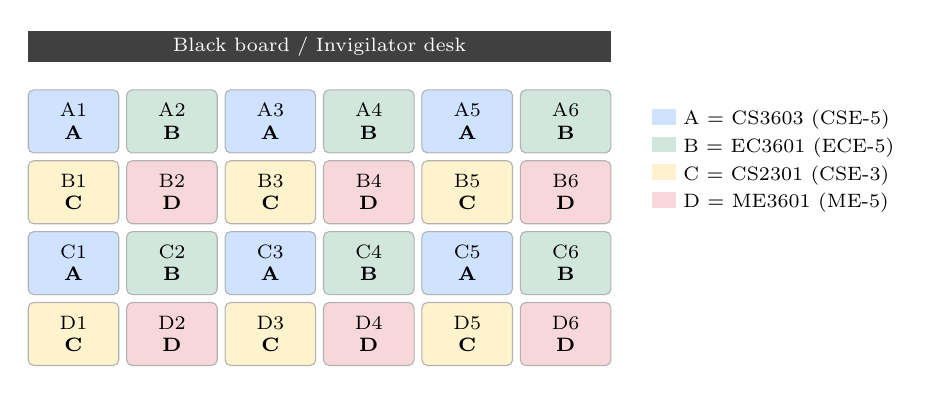
\begin{tikzpicture}[font=\scriptsize]
\definecolor{sA}{RGB}{207,226,255}
\definecolor{sB}{RGB}{209,231,221}
\definecolor{sC}{RGB}{255,243,205}
\definecolor{sD}{RGB}{248,215,218}
\fill[black!75] (0,0.35) rectangle (6*1.25-0.1,0.75);
\node[white] at (3.7,0.55) {Black board / Invigilator desk};
\foreach \s [count=\i from 0] in {A,B,A,B,A,B,C,D,C,D,C,D,A,B,A,B,A,B,C,D,C,D,C,D}{
  \pgfmathtruncatemacro{\r}{int(\i/6)}
  \pgfmathtruncatemacro{\c}{mod(\i,6)}
  \pgfmathtruncatemacro{\cc}{\c+1}
  \fill[s\s,draw=black!30,rounded corners=2pt] (\c*1.25,-\r*0.9) rectangle ++(1.15,-0.8);
  \node[align=center] at (\c*1.25+0.575,-\r*0.9-0.4) {\ifcase\r A\or B\or C\or D\fi\cc\\\textbf{\s}};
}
\node[anchor=west,align=left] at (7.8,-0.9) {
  \tikz\fill[sA](0,0)rectangle(0.3,0.2); A = CS3603 (CSE-5)\\[2pt]
  \tikz\fill[sB](0,0)rectangle(0.3,0.2); B = EC3601 (ECE-5)\\[2pt]
  \tikz\fill[sC](0,0)rectangle(0.3,0.2); C = CS2301 (CSE-3)\\[2pt]
  \tikz\fill[sD](0,0)rectangle(0.3,0.2); D = ME3601 (ME-5)};
\end{tikzpicture}

\caption{Illustrative seating pattern}
\end{figure}
\section{Invigilation Allocation}
After seating, the engine counts the students in each used hall and requires $\lceil s/30\rceil$ invigilators per hall. For each required invigilator it considers only faculty who have not reached their duty limit and have no duty overlapping the slot, and picks the one with the fewest duties so far. If nobody is free, the whole operation is rolled back.
\begin{figure}[H]\centering
\resizebox{!}{0.5\textheight}{\begin{tikzpicture}[
  font=\footnotesize, node distance=0.45cm,
  term/.style={rounded rectangle,draw=egnavy,fill=egnavy,text=white,minimum height=0.7cm,minimum width=3cm},
  proc/.style={rectangle,draw=egnavy,fill=eglight,rounded corners=2pt,minimum height=0.7cm,text width=5.6cm,align=center},
  dec/.style={diamond,draw=eggold,fill=eggold!20,aspect=2.6,inner sep=1pt,text width=2.6cm,align=center},
  err/.style={rectangle,draw=red!60!black,fill=red!8,rounded corners=2pt,text width=3.0cm,align=center,minimum height=0.7cm},
  arr/.style={-{Stealth[length=2mm]},thick}]
\node[term] (s) {Start (date, startTime)};
\node[dec,below=of s] (d0) {seating exists for slot?};
\node[err,right=0.8cm of d0] (e0) {throw Allocation\-Exception};
\node[proc,below=of d0] (p1) {Count students per hall; endTime = latest end time of exams in slot};
\node[proc,below=of p1] (p2) {Delete old duties of the slot; load all faculty and all existing duties};
\node[proc,below=of p2] (p3) {For each used hall: needed = $\lceil$students / 30$\rceil$ (minimum 1)};
\node[proc,below=of p3] (p4) {Candidates = faculty with duties $<$ maxDuties \textbf{and} no duty overlapping [startTime, endTime) on that date};
\node[dec,below=of p4] (d1) {any candidate?};
\node[err,right=0.8cm of d1] (e1) {throw Allocation\-Exception (rollback)};
\node[proc,below=of d1] (p5) {Choose candidate with fewest duties (tie: name order); create duty; update workload map};
\node[dec,below=of p5] (d2) {more seats to cover?};
\node[proc,below=of d2] (p6) {saveAll duties; return InvigilationResult};
\node[term,below=of p6] (e) {End};
\draw[arr] (s)--(d0);
\draw[arr] (d0)--node[above]{no}(e0);
\draw[arr] (d0)--node[right]{yes}(p1);
\draw[arr] (p1)--(p2); \draw[arr] (p2)--(p3); \draw[arr] (p3)--(p4); \draw[arr] (p4)--(d1);
\draw[arr] (d1)--node[above]{no}(e1);
\draw[arr] (d1)--node[right]{yes}(p5);
\draw[arr] (p5)--(d2);
\draw[arr] (d2)--node[right]{no}(p6);
\draw[arr] (d2.west) -- node[above]{yes} ++(-1.3,0) |- (p4.west);
\draw[arr] (p6)--(e);
\end{tikzpicture}
}
\caption{Invigilation allocation flowchart}
\end{figure}
\section{Complexity}
Seating runs in $O(P \cdot k)$ for $P$ seats and $k$ exams in a slot; invigilation runs in $O(I \cdot (|F| + D))$ for $I$ required invigilators, $|F|$ faculty and $D$ existing duties. Both are linear for practical purposes. Proofs of the constraints and a full worked example are in Document 03.

\chapter{Implementation}
\section{Project Structure}
\begin{lstlisting}[style=plain]
ExamGrid/
  pom.xml
  src/main/java/com/examgrid/
    ExamGridApplication.java
    config/  controller/api/  controller/web/  dto/  entity/
    exception/  repository/  security/  service/
  src/main/resources/
    application.properties
    templates/ (index, login, seat-lookup, admin/*, faculty/*, student/*, error/*)
    static/css/style.css   static/js/seat-lookup.js   static/js/table-filter.js
  src/test/java/com/examgrid/  (JUnit and MockMvc tests)
  docs/ (schema.sql, Postman collection, LaTeX reports)
\end{lstlisting}

\section{Modules}
\begin{tabularx}{\linewidth}{|L{3.4cm}|X|}
\hline\headrow\thead{Module} & \thead{Implementation}\\\hline
Entities & \texttt{Student}, \texttt{Faculty}, \texttt{Hall}, \texttt{Exam}, \texttt{SeatAllocation}, \texttt{InvigilationDuty}, \texttt{AppUser} with JPA and Bean Validation annotations; lazy many-to-one associations.\\\hline
Repositories & Interfaces extending \texttt{JpaRepository}; derived queries such as \texttt{findByBranchAndSemesterOrderByUsnAsc}; JPQL with \texttt{join fetch}; \texttt{@Modifying} bulk deletes.\\\hline
Services & CRUD services, the two allocation engines, \texttt{UserAccountService} and \texttt{ReportPdfService}.\\\hline
Web controllers & Form handling with \texttt{@Valid} and \texttt{BindingResult}; Post/Redirect/Get with flash attributes.\\\hline
REST controllers & JSON endpoints under \texttt{/api} returning entities or DTO records.\\\hline
Exception handling & Custom exceptions; \texttt{ApiExceptionHandler} and \texttt{WebExceptionHandler}.\\\hline
Security & Two \texttt{SecurityFilterChain} beans, \texttt{AppUserDetailsService}, BCrypt.\\\hline
Views & Thymeleaf layout fragments (head, navbar, alerts, footer), Bootstrap 5 WebJar, Spring Security dialect for role-based menus.\\\hline
\end{tabularx}

\section{Key Code}
\subsection{Entity with Validation}
\lstinputlisting[style=java,firstline=15,lastline=42,firstnumber=15,caption={Student entity (excerpt)}]{\src/entity/Student.java}

\subsection{Repository}
\lstinputlisting[style=java,firstline=14,lastline=47,firstnumber=14,caption={SeatAllocationRepository (excerpt)}]{\src/repository/SeatAllocationRepository.java}

\subsection{Seating Engine Core Loop}
\lstinputlisting[style=java,firstline=92,lastline=124,firstnumber=92,caption={Seat-by-seat placement in SeatingAllocationService}]{\src/service/SeatingAllocationService.java}

\subsection{Web Controller with Validation}
\lstinputlisting[style=java,firstline=43,lastline=63,firstnumber=43,caption={StudentWebController.save}]{\src/controller/web/StudentWebController.java}

\subsection{REST Controller}
\lstinputlisting[style=java,firstline=14,lastline=27,firstnumber=14,caption={SeatLookupApiController}]{\src/controller/api/SeatLookupApiController.java}

\subsection{Fetch API on the Client}
\lstinputlisting[language=Java,style=plain,firstline=36,lastline=56,firstnumber=36,numbers=left,numberstyle=\tiny\color{gray},caption={loadSeats in seat-lookup.js}]{../../src/main/resources/static/js/seat-lookup.js}

\subsection{Thymeleaf Seating Grid}
\lstinputlisting[style=plain,firstline=28,lastline=45,caption={Hall grid in admin/seating.html}]{../../src/main/resources/templates/admin/seating.html}

\chapter{REST API and Testing}
\section{REST Endpoints}
\begin{tabularx}{\linewidth}{|L{2.6cm}|X|L{2.8cm}|}
\hline\headrow\thead{Method} & \thead{Endpoint} & \thead{Access}\\\hline
GET, POST & /api/students, /api/faculty, /api/halls, /api/exams & ADMIN\\\hline
GET, PUT, DELETE & /api/\{resource\}/\{id\} & ADMIN\\\hline
GET & /api/exams/slots & ADMIN\\\hline
POST, GET & /api/allocations/seating?date=\&startTime= & ADMIN\\\hline
POST & /api/allocations/invigilation?date=\&startTime= & ADMIN\\\hline
GET & /api/seats/\{usn\} & public\\\hline
GET & /api/duties, /api/duties/workload & ADMIN\\\hline
GET & /api/duties/faculty/\{code\} & ADMIN, own FACULTY\\\hline
\end{tabularx}

\noindent Example:
\begin{lstlisting}[style=bash]
curl -u admin:admin123 -X POST "http://localhost:8080/api/allocations/seating?date=2026-12-07&startTime=09:30"
curl http://localhost:8080/api/seats/NNM24CS224
\end{lstlisting}
\begin{lstlisting}[style=json]
{ "examDate": "2026-12-07", "startTime": "09:30:00", "examsInSlot": 4,
  "studentsSeated": 148, "hallsUsed": 3, "adjacentSameSubjectPairs": 0 }
\end{lstlisting}
All endpoints with curl commands, request bodies, responses and error cases are documented in Document 04, and a ready Postman collection is provided in \texttt{docs/postman}.

\section{Testing}
\begin{tabularx}{\linewidth}{|l|X|c|}
\hline\headrow\thead{Test class} & \thead{Focus} & \thead{Tests}\\\hline
SeatingAllocationServiceTest & one seat per student, capacity, no same-subject neighbours, re-run, capacity error, empty slot, single-subject slot & 7\\\hline
InvigilationAllocationServiceTest & seating first, enough invigilators, no clash, balance, duty limit, 30-student rule, unknown faculty & 7\\\hline
ApiControllerTest (MockMvc) & public lookup, 404, 401/403/200, validation errors, own roster only, 422 & 6\\\hline
\end{tabularx}
\noindent The tests run with \texttt{mvn test} on an in-memory H2 database in MySQL mode with the sample data. In addition, 33 manual test cases (TC-01 to TC-44) cover the user interface, PDF export and mobile view; they are listed with a traceability matrix in Document 04.

\chapter{Results}
\section{Allocation Results on Sample Data}
\begin{table}[H]\centering
\caption{Seating results per slot (148 students, 4 halls, 192 seats)}
\begin{tabular}{|l|c|c|c|c|}
\hline\headrow\thead{Slot} & \thead{Exams} & \thead{Students} & \thead{Halls used} & \thead{Same-subject pairs}\\\hline
07-Dec 09:30 & 4 & 148 & SH-01, LH-201, LH-101 & 0\\\hline
08-Dec 09:30 & 3 & 108 & SH-01, LH-201 & 0\\\hline
08-Dec 14:00 & 1 & 40 & SH-01 (32), LH-201 (8) & 0\\\hline
\end{tabular}
\end{table}
\begin{table}[H]\centering
\caption{Invigilation results}
\begin{tabular}{|l|c|c|}
\hline\headrow\thead{Measure} & \thead{Manual process (typical)} & \thead{ExamGrid}\\\hline
Duties assigned (3 slots) & 14 & 14\\\hline
Time clashes & checked by eye & 0 (guaranteed)\\\hline
Workload spread (max $-$ min) & not tracked & 1\\\hline
Time to prepare & hours & under one second per slot\\\hline
\end{tabular}
\end{table}

\section{Screenshots}
\screenshot{01_home}{Home page}
\screenshot{02_login}{Login page}
\screenshot{03_admin_dashboard}{Exam cell dashboard}
\screenshot{04_students}{Student management with validation}
\screenshot{05_halls}{Hall management}
\screenshot{06_exams}{Exam timetable}
\screenshot{07_allocation}{Allocation page with exam slots}
\screenshot{08_seating_plan}{Generated seating plan (colour per subject)}
\screenshot{09_duties}{Invigilation duty roster and workload}
\screenshot{10_seating_pdf}{Seating chart PDF}
\screenshot{11_seat_lookup}{Public seat lookup by USN}
\screenshot{12_faculty_duties}{Faculty duty view}
\screenshot{13_postman}{Seat lookup API tested in Postman}
\screenshot{14_tests}{JUnit test results (mvn test)}

\chapter{Conclusion and Future Enhancements}
\section{Conclusion}
ExamGrid automates exam seating and invigilation allocation with a clean Spring Boot application. The rule-based engines satisfy all hard constraints -- every student seated once, hall capacity respected, no invigilator time clashes, duty limits honoured -- and in practice also achieve zero same-subject neighbours and an almost perfectly balanced invigilation workload. Students and faculty get self-service access to their allocations, and the exam cell gets printable charts and rosters from the same consistent data. The project gave us hands-on experience with the complete Spring ecosystem covered in CS3603-1: dependency injection, Spring MVC and Thymeleaf, Spring Data JPA with Hibernate and MySQL, Spring Security, Bean Validation, REST API design and centralized exception handling.

\section{Future Enhancements}
\begin{itemize}
  \item E-mail or SMS notification of seats and duties.
  \item Bulk import of students and timetable from CSV or Excel files.
  \item Support for students with special needs (ground-floor halls, extra time) and reserved seats.
  \item Rule to avoid assigning faculty to invigilate their own subject.
  \item QR code on admit cards linking to the seat lookup.
  \item Optional optimisation using constraint programming for very large or highly constrained sessions.
  \item Deployment on the college server with HTTPS and MySQL backups.
\end{itemize}

\begin{thebibliography}{9}
\bibitem{boot} Spring Boot Reference Documentation, version 3.3, VMware Tanzu. \url{https://docs.spring.io/spring-boot/}
\bibitem{sec} Spring Security Reference, version 6. \url{https://docs.spring.io/spring-security/reference/}
\bibitem{jpa} Spring Data JPA Reference Documentation. \url{https://docs.spring.io/spring-data/jpa/reference/}
\bibitem{thy} Thymeleaf 3.1 Documentation. \url{https://www.thymeleaf.org/documentation.html}
\bibitem{mysql} MySQL 8.0 Reference Manual, Oracle. \url{https://dev.mysql.com/doc/refman/8.0/en/}
\bibitem{openpdf} OpenPDF project. \url{https://github.com/LibrePDF/OpenPDF}
\bibitem{walls} C. Walls, \emph{Spring in Action}, 6th ed., Manning Publications, 2022.
\bibitem{ieee830} IEEE Std 830-1998, IEEE Recommended Practice for Software Requirements Specifications.
\bibitem{clrs} T. H. Cormen, C. E. Leiserson, R. L. Rivest and C. Stein, \emph{Introduction to Algorithms}, 4th ed., MIT Press, 2022 (greedy algorithms and graph colouring).
\end{thebibliography}

\appendix
\chapter{Installation and User Manual}
\section{Installation}
\begin{enumerate}
  \item Install JDK 17+, Maven 3.9 and MySQL 8. Start MySQL.
  \item Edit \texttt{src/main/resources/application.properties} if the MySQL user or password is not \texttt{root}/\texttt{root}.
  \item In the project folder run \texttt{mvn spring-boot:run}.
  \item Open \url{http://localhost:8080}. The database and sample data are created automatically.
\end{enumerate}
\section{Using the System}
\begin{enumerate}
  \item Log in as \texttt{admin} / \texttt{admin123}.
  \item Review or add halls, students, faculty and exams. New students and faculty can log in with their USN / code and the password \texttt{Welcome@123}.
  \item Open \emph{Allocation}. For each slot click \emph{1. Generate seating}, check the plan, then click \emph{2. Assign invigilators}.
  \item Download the seating chart from the plan page and the duty roster from the \emph{Duties} page.
  \item Students search their USN on \emph{Seat Lookup}; faculty log in and open \emph{My Duties}.
\end{enumerate}
\section{Companion Documents}
\begin{tabularx}{\linewidth}{|l|X|}
\hline\headrow\thead{Document} & \thead{Content}\\\hline
01\_Project\_Proposal\_and\_SRS & Proposal, schedule, IEEE SRS with numbered requirements\\\hline
02\_System\_Design\_and\_ERD\_Specification & Architecture, class and ER diagrams, data dictionary, security design\\\hline
03\_Allocation\_Algorithm\_and\_Backend\_Spec & Algorithms, proofs, worked examples, exception handling, security\\\hline
04\_REST\_API\_and\_Testing\_Report & All endpoints with curl and JSON, test plan, test cases, traceability\\\hline
05\_Final\_Lab\_Project\_Report & This report\\\hline
\end{tabularx}

\end{document}
